\part{Validation}

\chapter{Solution validation}

\section {Data model}

The model designed for the Observatory project represented in figure~\ref{fig:datamodel-obsproject} is a simplification of the ALMA Project Data Model summarized in section~\ref{sec:apdm} and it is the model used in the ALMA's Dynamic Scheduling Algorithm briefly described in section~\ref{sec:alma-dsa}.

The most relevant parts are: 
\begin{description}
\item[bla1] \hfill \\
Description of bla1
\end{description}

\begin{figure}[]	
\begin{center}
\includegraphics[width=1.15\textwidth]{images/ObsProject}
\caption{Observation Project data model}
\end{center}
\label{fig:datamodel-obsproject}
\end{figure}

The model designed for handle the observatory instrumentation is represented in figure~\ref{fig:datamodel-observatory}

\begin{figure}[]	
\begin{center}
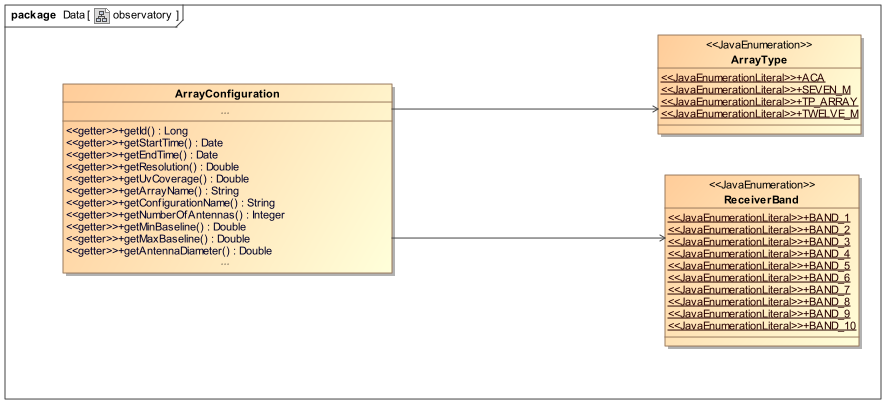
\includegraphics[width=\textwidth]{images/Observatory}
\caption{Observatory instrumentation data model}
\end{center}
\label{fig:datamodel-observatory}
\end{figure}

The model designed for handle the Executive information and the observing season is represented in figure~\ref{fig:datamodel-executive}

\begin{figure}[]	
\begin{center}
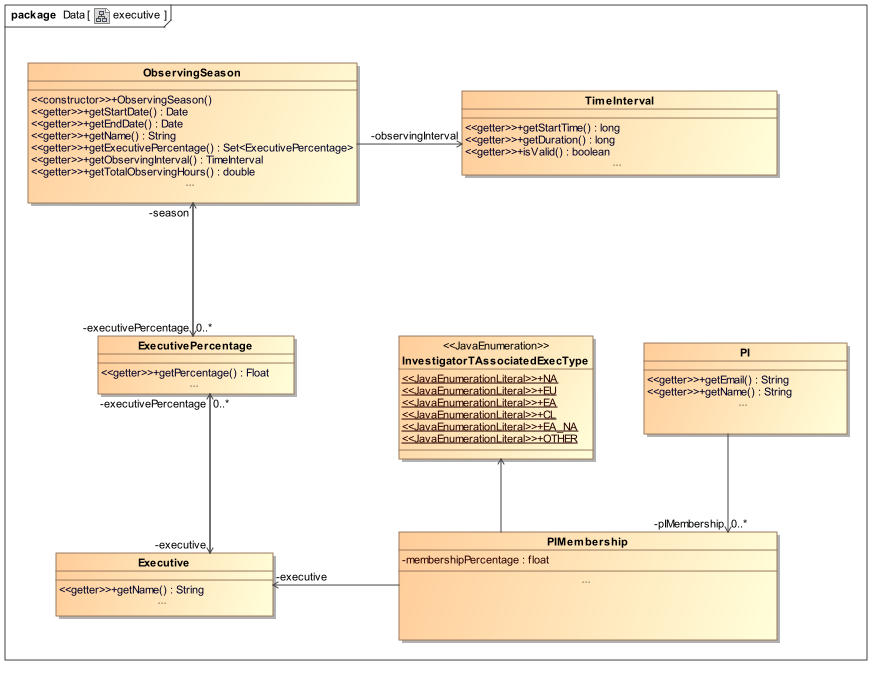
\includegraphics[width=\textwidth]{images/Executive}
\caption{Executive and observing season data model}
\end{center}
\label{fig:datamodel-executive}
\end{figure}

The model designed for handle the weather is represented in figure~\ref{fig:datamodel-weather}

\begin{figure}[]	
\begin{center}
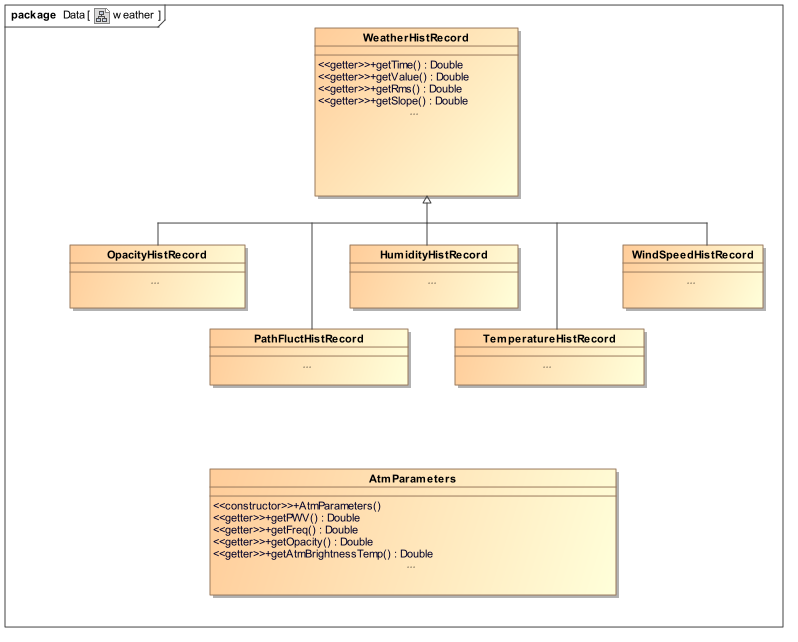
\includegraphics[width=\textwidth]{images/Weather}
\caption{Executive and observing season data model}
\end{center}
\label{fig:datamodel-weather}
\end{figure}

\section {Simulation}

\begin{figure}[]	
\begin{center}
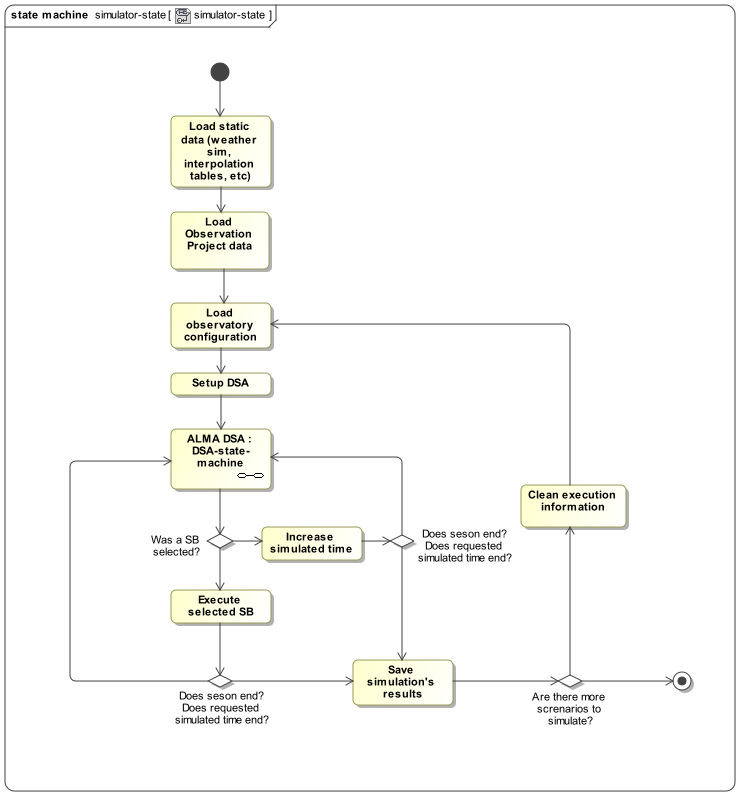
\includegraphics[width=\textwidth]{images/simulator-state-machine}
\caption{ALMA simulator's state machine}
\end{center}
\label{fig:sim-state-machine}
\end{figure}

\section {Algorithm implementation}

\section {Input Observation projects}

\begin{table}
\label{table:input-array-configs}
\begin{center}
\begin{tabular}{|c|c|c|c|}
\hline
Configuration name & Array type & Min. Baseline $[m]$ & Max. Baseline $[m]$\\
\hline
C34-1 & $12\,[m]$ & $14.2$ & $165.6$ \\
\hline
C34-2 & $12\,[m]$ & $14.1$ & $303.6$ \\
\hline
C34-3 & $12\,[m]$ & $20.6$ & $442.7$ \\
\hline
C34-4 & $12\,[m]$ & $20.6$ & $558.2$ \\
\hline
C34-5 & $12\,[m]$ & $25.8$ & $820.2$ \\
\hline
C34-6 & $12\,[m]$ & $40.6$ & $1091.0$ \\
\hline
C34-7 & $12\,[m]$ & $40.6$ & $1507.9$ \\
\hline
7m    & $7\,[m]$  & $8.9$  & $32.1$ \\
\hline
TP    & $TP$      & $-$    & $-$ \\
\hline
\end{tabular}
\end{center}
\caption{Array configurations provided as input for the algorithms}
\end{table}

\begin{figure}
        \centering
        \begin{subfigure}[b]{0.45\textwidth}
                \includegraphics[width=\textwidth]{images/c34-1_sources}
                \caption{C34-1} 
        \end{subfigure} 
        ~ %
%
        \begin{subfigure}[b]{0.45\textwidth}
                \includegraphics[width=\textwidth]{images/c34-2_sources}
                \caption{C34-2}
        \end{subfigure}

        \begin{subfigure}[b]{0.45\textwidth}
                \includegraphics[width=\textwidth]{images/c34-3_sources}
                \caption{C34-3}
        \end{subfigure}
        ~ 
        \begin{subfigure}[b]{0.45\textwidth}
                \includegraphics[width=\textwidth]{images/c34-4_sources}
                \caption{C34-4}
        \end{subfigure}% 
        
        \begin{subfigure}[b]{0.45\textwidth}
                \includegraphics[width=\textwidth]{images/c34-5_sources}
                \caption{C34-5}
        \end{subfigure}
        ~
        \begin{subfigure}[b]{0.45\textwidth}
                \includegraphics[width=\textwidth]{images/c34-6_sources}
                \caption{C34-6}
        \end{subfigure}
        
        \begin{subfigure}[b]{0.45\textwidth}
                \includegraphics[width=\textwidth]{images/c34-7_sources}
                \caption{C34-7}
        \end{subfigure}           
        \caption{Visibility of A-graded Scheduling Blocks for $12\,[m]$ Array Configurations}\label{fig:results-sb-critical-set}
\end{figure}